\section{Early Deposition Swaption}
\label{app:conv-swaption}

This type of swaption is the conventional form that is first introduced in \cite{liu2018atomic}. We rebuild this type with our meta-swaption extended form in the way depicted in Fig~\ref{fig:swaption-early-deposition}. Moreover, we begin analysing each stage of this type by explaining every possible scenarios which is mentioned in \ref{app:conv-swaption}

\begin{itemize}
    \item \textbf{Contract Funding}: Alice and Bob broadcast their funding transactions. Alice's includes margin and premium and Bob's include margin worth as equal to Alice's margin.
    
    \item \textbf{Principal Deposition}: In this stage, Bob is waiting for Alice to deposit her principal. Two scenarios:
    \begin{itemize}
        \item Alice does not deposit her principal. In this case, Bob also defaults and their margins are exchanged.
        \item Alice deposits her principal but Bob does not. In this case, Alice is in option contract stage. So, she reveals \Atwo and takes Bob
    \end{itemize}
     But if Bob fails to deposit his principal, Alice is already in option contract stage and she can take the ownership of both her principal and Bob's margin by revealing the \Atwo key and broadcasting Bob's default transaction.
    
    \item \textbf{Option Contract}: If both parties go to this stage, Alice can then use her option as mentioned earlier.
\end{itemize}

\begin{figure*}
    \centering
    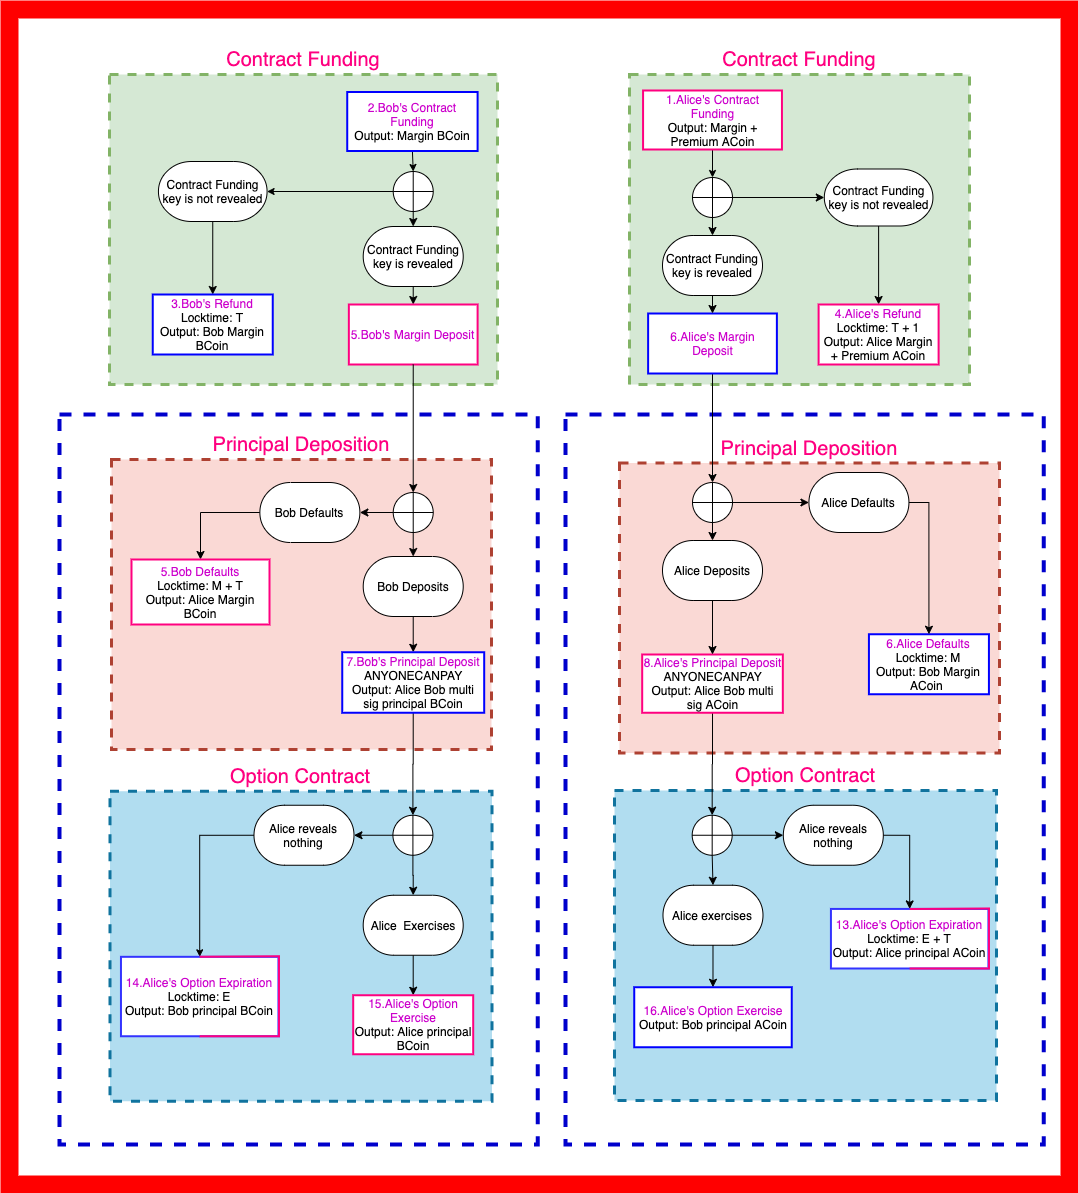
\includegraphics[width=\textwidth]{figures/conventional-swaption.png}
    \caption{Early Deposition swaption where the buyer (Alice) deposits her principal earlier than the seller (Bob). The pink-bordered transactions are broadcasted by Alice and the blue-bordered ones by Bob.}
    \label{fig:swaption-early-deposition}
\end{figure*}
%\ahC{Shall we mention that 546 Satoshis can %not be counted as margin?}
\section{Margin-Free Swaption}

\label{app:margin-free-swaption}
Until now, it was believed that Alice's margin deposit is necessary due to the limitations of HTLCs \cite{liu2018atomic}. In this work we propose a novel approach which allows Alice to participate in a swaption without depositing any margin.
In the beginning of contract Bob deposits an amount of BCoin as guarantee which is sent to Alice directly by revealing \Aone key. Alice also adds an amount of ACoin equal to Bob's guarantee to her premium, though non of them will directly sent to Bob. Later the premium and guarantee go to Bob in all possible situations except where Bob refuses to reveal the \keyone key when Alice does not default, then he will be punished by not paying back his guarantee.
% In Fig~ \ref{fig:swaption-margin-free-limited} we use our getting a guarantee money from Bob to build the {\it Margin Free} swaption.
% In this type besides premium, Alice deposits an amount of ACoiun equal to Bob's guarantee. Her premium is not paid directly after revealing of \Aone key, but instead will be locked until Bob acts honestly up to end of the Leader Lock stage.
% Later the premium goes to Bob in all possible situations except where Bob refuses to reveal the \keyone key and he will be punished by not paying back his guarantee. 
The amount of guarantee can be vary depends on the Alice's need.
If this type of swaption is used lonely without further contracts, the minimum valuable amount is enough (Even if it is less than premium) for the amount of guarantee. However, to use it alongside other contracts, Alice needs to set the guarantee value of Bob more than the summation of all the premiums which she wants to spend in her later contracts. Otherwise Bob is incentivized to pretend himself as the other parties in later contracts and cheats on Alice by stealing Alice's premiums in the later swaptions by not exposing the \keyone key and loosing his guarantee. Note that if Bob acts honestly, the guarantees in both sides will be exchanged.

\begin{itemize}
    \item \textbf{Contract Funding}: Bob pays his margin plus an amount of guarantee which prevents him from cheating in later stages. Alice also pays extra premium which in the case of Bob's honest behaviour pays back the guarantee to Bob. Guarantee in the Bob's section is directly send to Alice after revealing the \Aone key. 
    
    \item \textbf{Principal Deposition}: This stage is the same as previous principal deposition stages for Bob. He has M locktime to deposit his principal. If he does not, Alice takes his margin. In Alice's section, either she defaults and gives Bob the premium or she deposits her principal and goes to the next stage waiting for Bob to reveal the \keyone key.
    % \item \textbf{Premium Guarantee}: Either Alice defaults and gives Bob the premium or she deposits her principal and goes to the next stage waiting for Bob to reveal the \keyone key.
    
    \item \textbf{Leader Key}: If Bob has not deposited his principal until M locktime, Alice will also avoid depositing her principal and give Bob the premium and ACoin guarantee while gets his Margin from him.
    % and Alice has two options ahead: 1)She deposits her principal before M + T, then broadcasts the \keyone key expiration transaction, in which her premium is refunded. Therefore, if Bob defaults and Alice does not, there would be no premium for Bob. In any other situation he gets the premium. 
    If both parties have deposited their principals when this stage begins, Bob's decision whether to reveal the \keyone key or not, determines the fate of the swaption. If he refuses to reveal, he takes his own money back and Alice takes her own money including premium back. In this case, Bob loses his guarantee as a punishment. Otherwise, if he reveals the \keyone key, they both go to the next stage waiting for Alice to exercise her option. Additionally, by revealing the \keyone key, Bob finishes his task and it is the time to send back his guarantee. Hence at the end of this stage, Bob's guarantee will be paid back to himself.
    
    \item \textbf{Option Funding}: This stage is similar to the last versions of swpation.
\end{itemize}

\begin{figure*}
    \centering
    \includegraphics[height= 650 px]{figures/margin-free-limited-swaption.png}
    \caption{Margin free limited swpation where the buyer (Alice) is not supposed to deposit any margin. Pink-bordered transactions are broadcasted by Alice and blue-bordered ones by Bob.}
    \label{fig:swaption-margin-free-limited}
\end{figure*}
\fatemeC{mention auction as an application for the margin-free swaption. you can use the aucion section primarily written}